% Start here


\chapter{Introduction}
\label{sec:intro}


The aim of this document is to report the results of the task T7.1 of WP7:  "Primary tool Chain analyses and recommendations".

\section{Executive Summary}

Three tool chains have been proposed, which will be referred to with the following shortcuts for brevity:

\begin{description}
\item[Scade.] This tool chain is based on Scade in connection with Papyrus, for which an integration already exisists.

\item[EFS.] This tool chain is based on ERTMS Formal Specs (EFS), in connection with Papyrus, for which an integration has to be developed.  It will take advantage of elements from the Eclipse Ecosystem (and from Topcased, wherever possible).  The methods for integrating the various models have to be developed, as well as the gluing code that will hold everything together.

\item[B.] This tool chain is based on B in connection with Papyrus, for which an integration has to be developed.

\end{description}

\section{T7.1 Objective}

The goal of WP7 is to provide other openETCS workpackages with tooling for their activities.  Tools have been separated into primary and secondary tooling.  Task T7.1 is concerned with the identification of the best primary tooling, considering all constraints of the project.  Selecting tools also entails selecting modeling languages and an integration platform.

 \begin{figure}[b!]
  \centering
  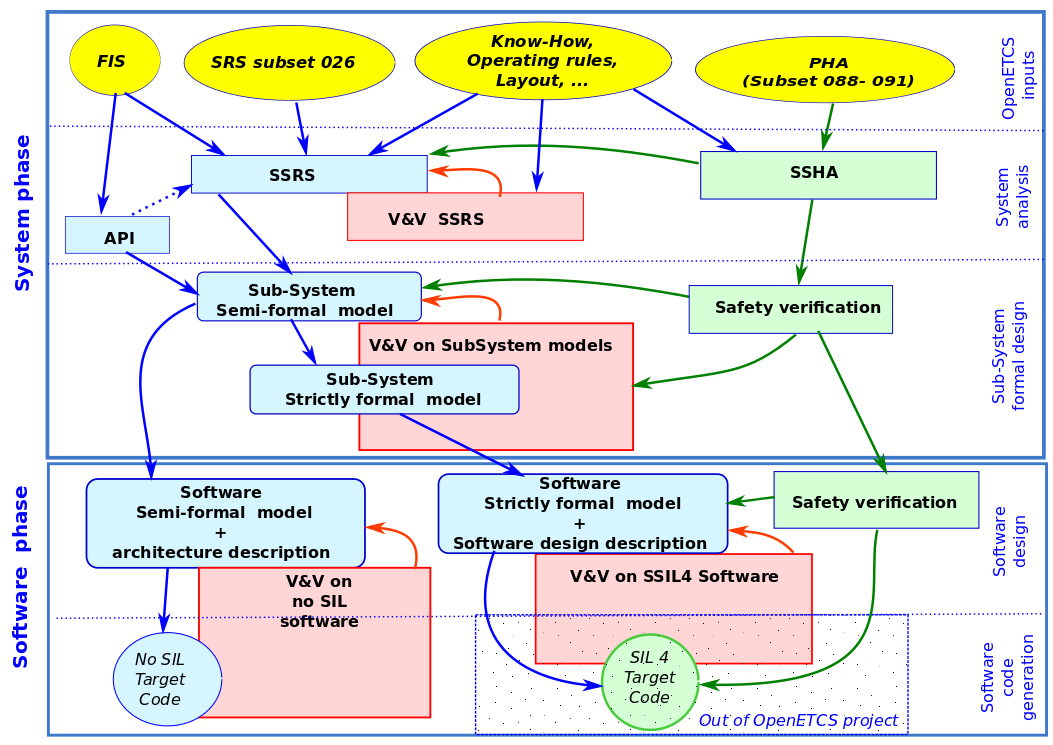
\includegraphics[scale=0.45]{images/WholeProcess.png}
  \caption{Main OpenETCS process.  The models that are covered by primary tooling are shown in blue.}
  \label{fig:main_process}
\end{figure}


\section{Scope of Task T7.1}

The scope of the primary tooling has been defined in the WP7 Description of Work \cite{}.  Figure~\ref{fig:main_process} depicts the main process (from D2.3).  In the scope of the primary tooling are (according to the DoW):

\begin{description}
  \item [Sub-System Semi-formal model.]  ``A semi-formal model of the system specification is defined from the SSRS. This model shall reflect the architecture defined in SSRS. (...) The semi-formal model shall be as consistent as possible with the SSRS level of abstraction, in particular choices concerning
software architecture and design have not to be described at this level. In practice, all the requirements of SSRS and of the sub-system Hazard analysis shall be covered by the semi-formal model.'' (D2.3, 4.4.3).  ``The means of description of the semi-formal model shall be understandable by domain experts, providing graphical description'' (D2.3, 4.4.4).

  \item [Sub-System Strictly formal model.] ``This semi-formal model \emph{can} be extended with strictly formal models to improve the understanding of some part of the sub-system.'' (D2.3, 4.4.2).  ``To facilitate safety activities, the safety relevant function should be as much as possible insulated from non safety relevant functions.'' (D2.3, 4.4.3).

  \item [Software Semi-formal model + architecture description.] The main output of this step is a semi-formal model which allows to produce executable code. ``This model shall be completed by a Software Architecture and Design Specification, which describes the software architecture and the design choices. (...) The semi-formal model defined during the system phase shall be completed, keeping the same language or extending it to cover specific software aspects.'' (D2.3, 4.5.2).

  \item [Software Strictly formal model + Software design description.]  This model is concerned with the functional and safety branch.  This activity ``shall provide methods and a toolchain to obtain SIL4 executable code of the on-board software application.'' (D2.3, 4.5.3).

\end{description}

\subsection{Scope with respect to SSRS, API and code}

API, Code and SSRS\footnote{Note that the DoW does not even mention the SSRS, as its creation has been proposed the first time in February 2013, when the DoW was already finalized.  Therefore, we include SSRS-related activities with T7.2.3 (Requirement traceability) and report on them in O7.2.5 (Requirement management tool choices).}  are in the scope of the secondary toolchain (T7.2).  Of course, choices in the primary tool chain that may affect the secondary tool chain will be covered in this document.

The SSRS poses a special challenge, as activities in its creation have already started.  Even though no tools have been selected yet.  Deliverable D2.3 describes the form of the SSRS as follows:
``The SSRS (...) shall be described as textual documents.'' (4.3.4).  It continues to state: ``However these documents shall be completed by a semi-formal model to describe the functional architecture of the on-board unit''.

The connection between SSRS and Sub-System Semi-formal model is described as: ``A semi-formal model of the system specification is defined from the SSRS. (...) In practice, all the requirements of SSRS and of the subsystem Hazard analysis shall be covered by the semi-formal model.''

There is even less information regarding the API, except that it is handled corresponding to the SSRS: ``The SSRS and API shall be described as textual documents. However these documents shall be completed by a semiformal model to describe the functional architecture of the on-board unit.'' (D2.3, 4.3.4).

There is little relevant information with regard to code generation in this report, except that it makes some implications regarding the software functional model: ``A first executable code is produced from the software functional model.  This executable code shall be non vital. However it shall be able to run in real time on a on-board computer.  Thus it shall comply to the standardised interfaces.'' (D2.3, 4.6.2).

%The objectives of this task are to identify the modelling languages, the tools and the tool platform suitable to define the primary tool chain of OpenETCS project. This primary tool chain shall  cover all specification and design activities of the OpenETCS process (part in blue in \ref{fig:main_process}). For more details see D2.3 \citep{D2_3} and D2.6-9 \citep{D2_6}. Means and tools for other activities described on figure \ref{fig:main_process} (mainly verification, validation and safety activities)  are going to be discussed during the task T7.2 of WP7.

\section{Organization of this Report}

This report is organized as follows:

\begin{description}
\item[Introduction (Section \ref{sec:intro}).] An executive summary, as well as an overview of the WP7 Task T7.1 activities.  It shows how T7.1 fits into openETCS in general and WP7 in particular.  It also describes the scope of the results described in this deliverable, making sure the boundary to the secondary tool chain is properly defined.

\item[Results on Means and Tools (Section \ref{sec:results}).] A description of the three proposed tool chains.  The selection process is described in detail.

\end{description}

%\section{T7.1 activities}

%The activities have started in November 2012, with the completion of the WP7 DoW and consequently the organization of the benchmark.  

%After selection of a set of case studies (specified in D2.5 \citep{D2_5}), different approaches have been proposed and models have been stored on a common open github repository. All the methods have been presented during a public meeting in April 2013.

%Besides, a set of criteria have been defined according the D2.6-9 requirement document \citep{D2_6}.  The results are recorded in the outputs O7.1.3-O7.1.7 \citep{WP7_O713_O717} for means and tools and O7.1.9 \citep{WP7_O719} for tool platform.

%A decision meeting took place the 4th of July 2013 to analyze the results of the benchmark and to decide which means and tools will be retained during the process.

%Results of the decision are given in this current document. 



%%%%%%%%%%%%%%%%%%%%%%%%%%%%%%%%%%%%%%%%%%%%%%%%%%%%%%%%%%%%%%%

\section{Glossary}
\label{sec:glossary}

\begin{description}
\item[API] Application Programming Interface
\item[DoW] Description of Work.  In this document we typically mean the WP7 DoW.
\item[FIS] Functional Interface Specification
\item[HW] Hardware
\item[I/O] Input/Output
\item[OBU] On-Board Unit
\item[PHA] Preliminary Hazard Analysis
\item[SIL] Safety Integrity Level
\item[SRS] System Requirement Specification
\item[SSHA] Sub-System Hazard Analysis
\item[SSRS] Sub-System Requirement Specification
\item[SW] Software
\item[V\&V] Verification \& Validation
\end{description}

%%%%%%%%%%%%%%%%%%%%%%%%%%%%%%%%%%%%%%%%%%%%%%%%%%%%%%%%%%%%%%%


